%
% einleitung.tex -- Beispiel-File für die Einleitung
%
% (c) 2020 Prof Dr Andreas Müller, Hochschule Rapperswil
%
% !TEX root = ../../buch.tex
% !TEX encoding = UTF-8
%
%\section{Teil 0\label{step:section:teil0}}
%\kopfrechts{Teil 0}
%Lorem ipsum dolor sit amet, consetetur sadipscing elitr, sed diam
%nonumy eirmod tempor invidunt ut labore et dolore magna aliquyam
%erat, sed diam voluptua \cite{step:bibtex}.
%At vero eos et accusam et justo duo dolores et ea rebum.
%Stet clita kasd gubergren, no sea takimata sanctus est Lorem ipsum
%dolor sit amet.
%
%Lorem ipsum dolor sit amet, consetetur sadipscing elitr, sed diam
%nonumy eirmod tempor invidunt ut labore et dolore magna aliquyam
%erat, sed diam voluptua.
%At vero eos et accusam et justo duo dolores et ea rebum.  Stet clita
%kasd gubergren, no sea takimata sanctus est Lorem ipsum dolor sit
%amet.


%\chapter{Differentiation in Simulationen – Complex Step und Automatic Differentiation}

\section{Klassische Finite Differenzenmethode}
\kopfrechts{Klassische Finite Differenzenmethode}
%Die numerische Approximation von Ableitungen basiert wesentlich auf der Taylor-Reihe, 
%welche das lokale Verhalten einer Funktion in der Umgebung eines Entwicklungspunktes $a$ wie folgt beschreibt
%\begin{equation}
%	f(x) = \sum_{k=0}^{\infty} \frac{\left(x-a\right)^k}{k!}f^{(k)}\left(a\right).
%\end{equation}
%Für eine hinreichend oft differenzierbare Funktion $f$ lässt sich der Funktionswert 
%an einer nahegelegenen Stelle $x+h$ durch eine endliche Summe von Ableitungen an der 
%Stelle $x$ darstellen:
%
%\begin{equation}
%	f(x+h) = \sum_{k=0}^{n} \frac{h^k}{k!} f^{(k)}(x) + E_n(h).
%\end{equation}

Für eine hinreichend oft differenzierbare Funktion $f$ lässt sich der Funktionswert 
in der Umgebung eines Punktes $x$ mithilfe der Taylor-Entwicklung darstellen. 
Ausgehend von der allgemeinen Taylorreihe um einen Entwicklungspunkt $a$

\begin{equation}
	f(x) = \sum_{k=0}^{\infty} \frac{(x-a)^k}{k!} f^{(k)}(a),
	\label{step:taylor1}
\end{equation}
kann der Funktionswert an einer nahegelegenen Stelle $x+h$ bestimmt werden, indem 
zunächst der Auswertungspunkt verschoben wird, d.\,h.\ es wird $x \mapsto x+h$ gesetzt. 
Damit ergibt sich

\begin{equation*}
	f(x+h) = \sum_{k=0}^{\infty} \frac{((x+h)-a)^k}{k!} f^{(k)}(a).
\end{equation*}

Wählt man nun den Entwicklungspunkt gleich dem Referenzpunkt, also $a = x$, so wird 
die Taylorreihe gezielt um den Punkt $x$ entwickelt. Dies ist insbesondere deshalb 
sinnvoll, da die Ableitungen der Funktion an der Stelle $x$ ausgewertet werden und 
somit eine lokale Beschreibung der Funktion in der Umgebung von $x$ erfolgt.
Durch diese Wahl vereinfacht sich der Ausdruck im Argument der Potenzterme zu
\[
(x+h) - a = (x+h) - x = h,
\]
sodass der Abstand zwischen Entwicklungs- und Auswertungspunkt direkt durch die 
Schrittweite $h$ beschrieben wird. Gleichzeitig werden die Ableitungen an der Stelle 
$a$ durch Ableitungen an der Stelle $x$ ersetzt, also $f^{(k)}(a) = f^{(k)}(x)$.
Damit ergibt sich eine Darstellung des Funktionswertes $f(x+h)$ ausschliesslich in 
Abhängigkeit von den Ableitungen an der Stelle $x$ sowie der Verschiebung $h$, was 
insbesondere für numerische Verfahren von Vorteil ist, da nur lokale Informationen 
benötigt werden.
Man erhält somit die Entwicklung
\begin{equation}
	f(x+h) = \sum_{k=0}^{\infty} \frac{h^k}{k!} f^{(k)}(x).
			\label{step:taylor2}
\end{equation}

In der praktischen Anwendung wird diese unendliche Reihe nach endlich vielen Gliedern 
abgebrochen, sodass sich die Darstellung
\begin{equation*}
	f(x+h) = \sum_{k=0}^{n} \frac{h^k}{k!} f^{(k)}(x) + E_n(h)
			\label{step:finiteDifferenz}
\end{equation*}
ergibt, wobei $E_n(h)$ den Restterm bezeichnet, der den Fehler durch das Abschneiden 
der Reihe beschreibt. Für ein hinreichend kleines $h$ liefert diese endliche Summe eine 
gute Approximation des Funktionswertes $f(x+h)$.
Diese Darstellung zerlegt die Funktion in eine Folge zunehmend genauerer Approximationen. 
Der erste Term $f(x)$ beschreibt den Funktionswert selbst, während der lineare Term 
$f'(x)h$ die lokale Steigung berücksichtigt.
Höhere Ableitungen erfassen zusätzlich 
Krümmung und feinere Struktureigenschaften der Funktion. Mit wachsender Ordnung $n$ 
verbessert sich die Genauigkeit der Approximation systematisch.
Mit genügend klein gewählter Schrittweite $h$ können die Terme höherer Ordnung sogar vernachlässtigt werden.

\subsection{Der Restterm und seine Bedeutung}

Die Genauigkeit der Taylor-Approximation wird durch den Lagrange-Restterm
\begin{equation*}
	E_n(h) = \frac{h^{n+1}}{(n+1)!} f^{(n+1)}(\xi)
\end{equation*}
charakterisiert, wobei $\xi$ zwischen $x$ und $x+h$ liegt. Dieser Term beschreibt die 
Abweichung zwischen der exakten Funktion und ihrer Approximation durch ein Polynom 
vom Grad $n$.

Der Restterm liefert mehrere wichtige Einsichten:
\begin{itemize}
	\item Die Approximation wird für kleine Schrittweiten $h$ genauer.
	\item Die Genauigkeit steigt mit der Ordnung der Entwicklung.
	\item Das Verhalten der höheren Ableitungen beeinflusst massgeblich den Fehler.
\end{itemize}
Insbesondere zeigt die Abhängigkeit von $h^{n+1}$, dass der Fehler für kleine $h$ 
sehr schnell gegen Null konvergiert, sofern die Ableitungen beschränkt bleiben.

\subsection{Herleitung numerischer Ableitungen}

Betrachtet man die Entwicklung der Taylor-Reihe bis zur ersten Ordnung,

\begin{equation*}
	f(x+h) = f(x) + h f'(x) + \frac{h^2}{2!}f''(\xi),
\end{equation*}
so ergibt sich durch Umstellen eine Approximation für die erste Ableitung
\begin{equation}
	f'(x) \approx \frac{f(x+h) - f(x)}{h}.
	\label{step:finitdiff}
\end{equation}
Der zugehörige Fehler ist von der Ordnung $\mathcal{O}(h)$, was direkt 
aus dem Restterm der Taylor-Entwicklung folgt
\begin{equation*}
	\mathcal{O}(h) = \frac{h}{2}f''(\xi).
\end{equation*}
Diese sogenannte Vorwärtsdifferenz stellt die einfachste numerische Näherung der 
Ableitung dar.
Als Pendant zur Vorwärtsdifferenz lässt sich auch die Rückwärtsdifferenz bilden, indem $h<0$ gewählt wird:

\begin{equation*}
	f'\left(x\right) \approx \frac{f\left(x\right) - f\left(x-h\right)}{h},
	\label{step:diffmethod}
\end{equation*}
wobei auch diese Approximation einen Fehler erster Ordnung von $\mathcal{O}(h)$ aufweist.
Durch geschickte Kombination mehrerer Taylor-Entwicklungen lassen sich Approximationen verschiedener Ordnung bilden. 
Beispielsweise können die beiden Entwicklungen
\begin{equation*}
	f\left(x+h\right) = f\left(x\right) + h f'\left(x\right) + \frac{h^2}{2!}f''\left(x\right) + \frac{h^3}{3!}f'''\left(\xi_1\right), \quad\xi_1 \in \left(x , x + h\right)
\end{equation*}

\begin{equation*}
	f(x-h) = f(x) - h f'\left(x\right) + \frac{h^2}{2!}f''\left(x\right) - \frac{h^3}{3!}f'''\left(\xi_2\right), \quad\xi_2 \in \left(x , x + h\right)
\end{equation*}
voneinander subtrahiert werden, was folgenden Term ergibt
\begin{equation*}
	f\left(x+h\right) - f\left(x-h\right) =  2h f'\left(x\right) + h^3 \frac{f'''\left(\xi_1\right) + f'''\left(\xi_2\right)}{6}.
\end{equation*}
Somit gilt für die Ableitung 
\begin{equation*}
	f'\left(x\right) \approx \frac{f\left(x + h\right) - f\left(x-h\right)}{2h},
\end{equation*}
mit einem Fehlerterm
\begin{equation*}
	\mathcal{O}(h^2) = h^2\frac{f'''\left(\xi_1\right) + f'''\left(\xi_2\right)}{12}.
\end{equation*}
Man spricht hierbei von der zentrierten Differenzapproximation. 
Natürlich sind auch Differenzapproximationen höherer Ordnung möglich, dazu müssen lediglich mehr Terme (bpsw. $f\left(x + h\right), f\left(x - h\right), f\left(x + 2h\right), f\left(x - 2h\right)$) berücksichtigt werden. 


%In wissenschaftlichen und ingenieurtechnischen Anwendungen kommt es häufig vor, dass keine exakte Formel für $ f\left(x\right) $ bekannt ist.
%Stattdessen stehen möglicherweise nur eine Menge von Datenpunkten 
%\begin{equation}
%(x_1, y_1), (x_2, y_2), \ldots, (x_n, y_n)
%\end{equation}
%zur Verfügung, um die funktionale Abhängigkeit $ y = f\left(x\right) $ zu beschreiben.
%
%Wenn in einer solchen Situation die Änderungsrate von $ y $ in Bezug auf $ x $ abgeschätzt werden muss, können die oben beschriebenen Differenz-Formeln verwendet werden, um Näherungen für die Ableitung $ f'(x) $ zu berechnen.




\subsection{Fehleranalyse und Interpretation der numerischen Ergebnisse}

Zur Veranschaulichung der zuvor hergeleiteten Differenzapproximationen wird der absolute Fehler in Abhängigkeit von der Schrittweite $h$ in einem doppelt-logarithmischen Diagramm dargestellt.
\begin{figure}[h!] %todo
	\centering
	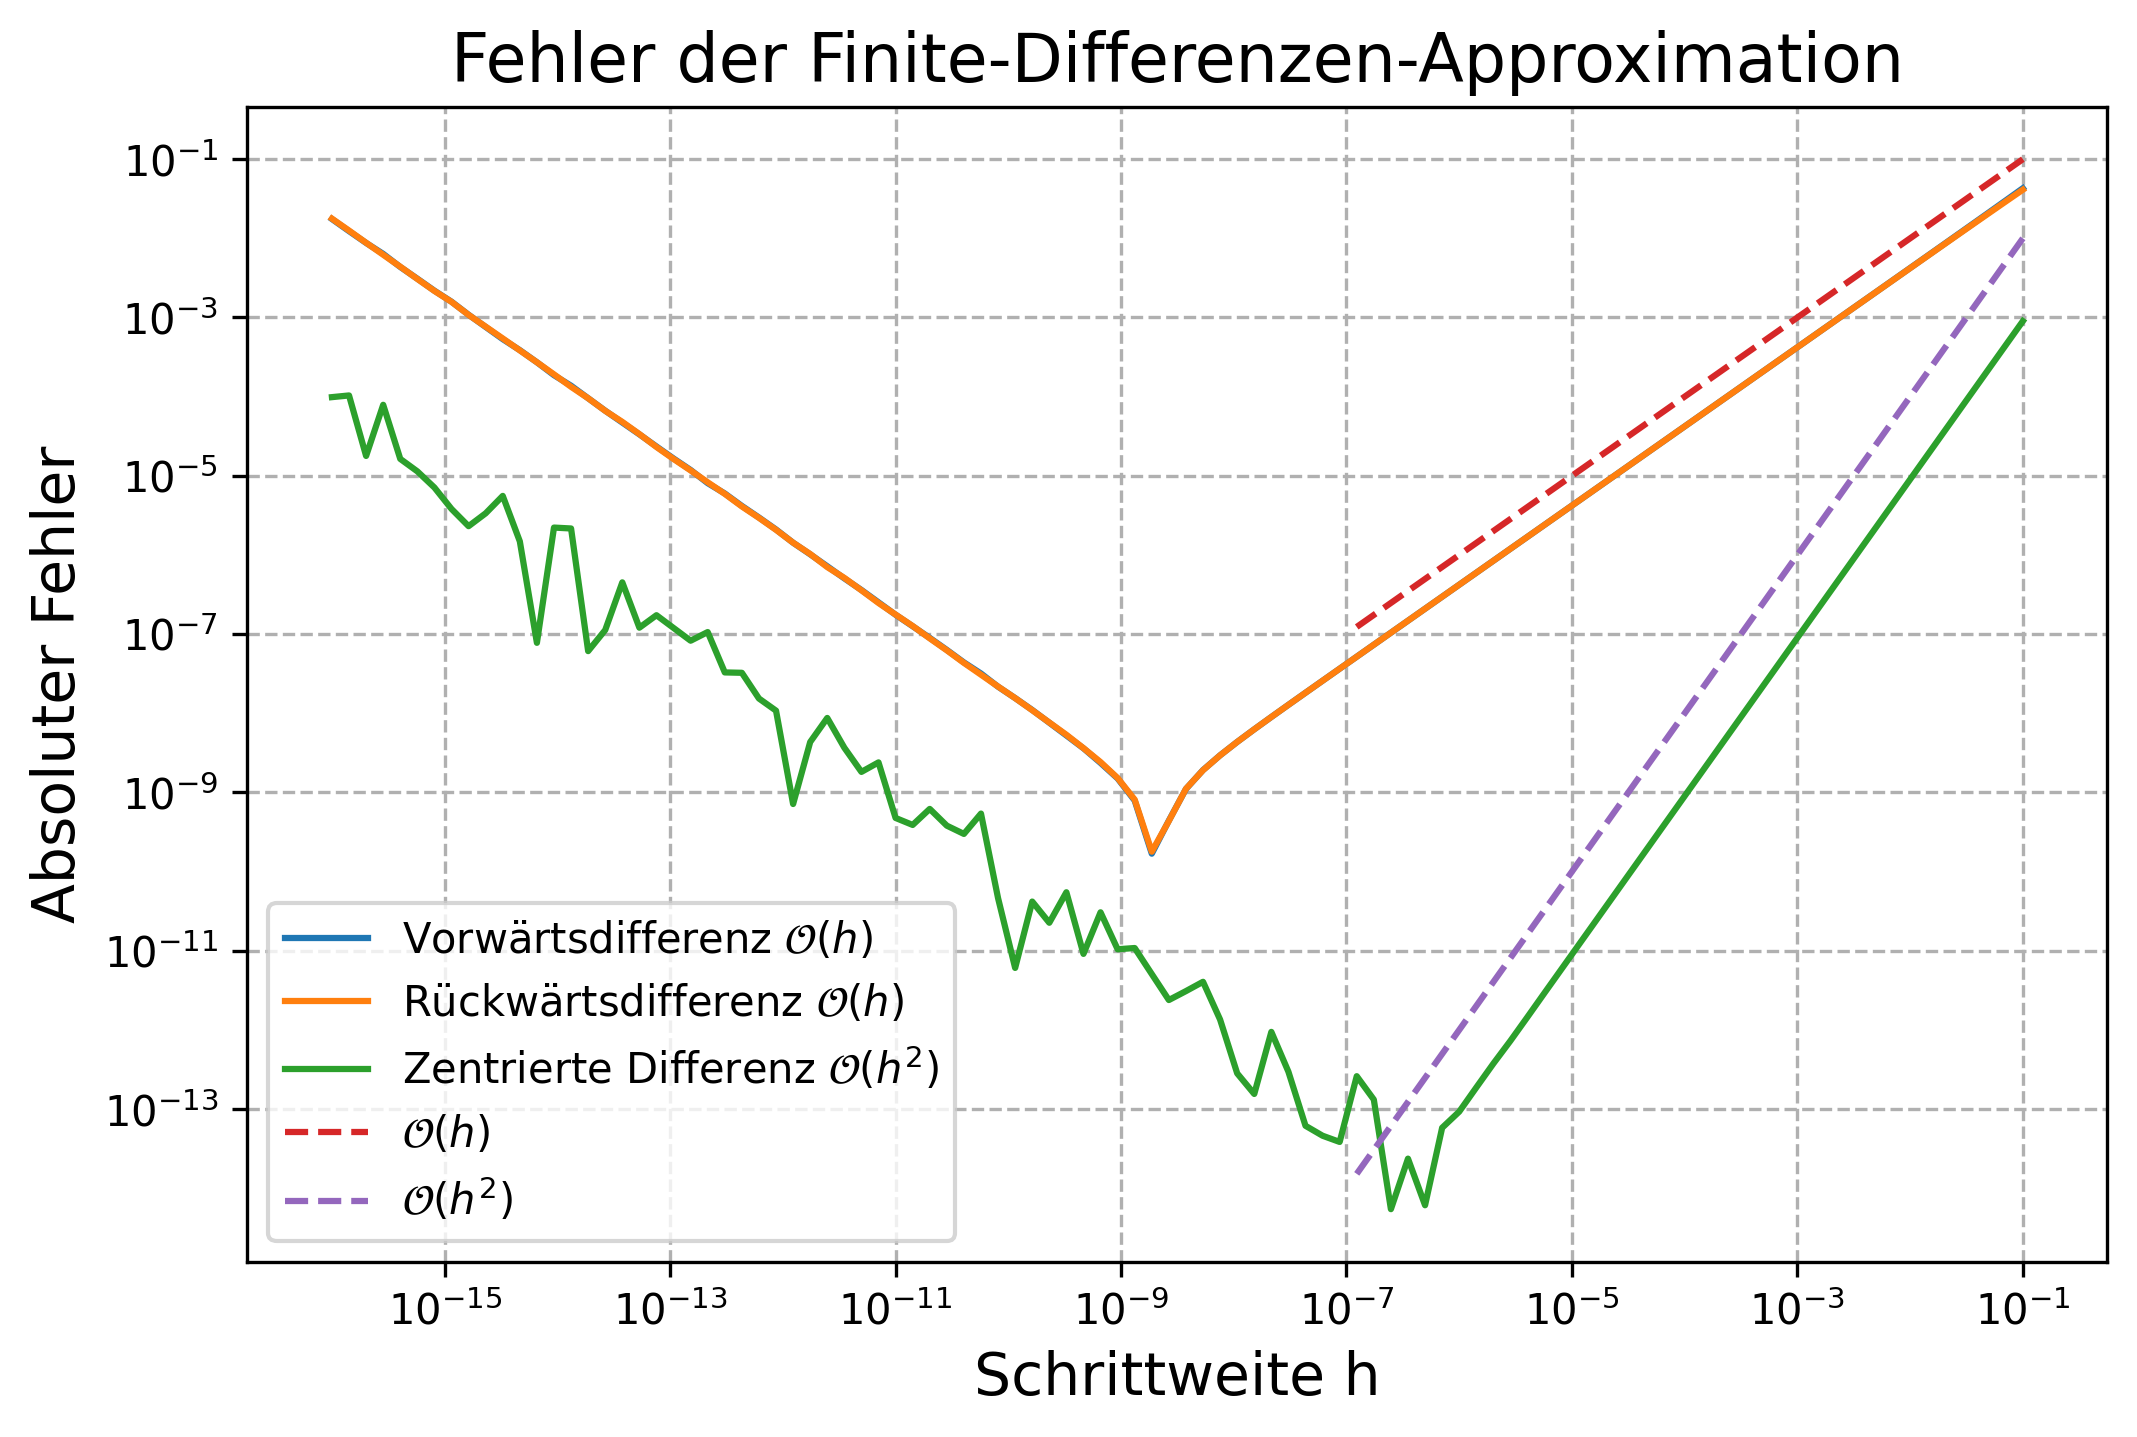
\includegraphics[width=0.8\textwidth]{papers/step/img/finite_differenzen_vergleich.png}
	\caption{Logarithmische Darstellung des absoluten Fehlers der Vorwärts-, Rückwärts- und zentrierten Differenz in Abhängigkeit von der Schrittweite $h$.}
	\label{fig:fehler_finite_differenzen}
\end{figure}
Abbildung \ref{fig:fehler_finite_differenzen} zeigt den Verlauf des absoluten Fehlers der verschiedenen Differenzapproximationen in Abhängigkeit der Schrittweite $h$.
Im rechten Bereich der Abbildung, d.\,h. für grössere Schrittweiten, dominiert der Diskretisierungsfehler, welcher aus dem Abbruch der Taylor-Reihe resultiert.
In diesem Bereich zeigt sich das erwartete asymptotische Verhalten der Approximationen. Die Vorwärts- und Rückwärtsdifferenz weisen eine lineare Abhängigkeit vom Parameter $h$ auf,
\begin{equation*}
\lvert E \rvert \sim \mathcal{O}(h),
\end{equation*}
was sich im Log-Log-Diagramm durch eine Gerade mit Steigung $1$ äussert. Die zentrierte Differenz hingegen besitzt ein quadratisches Fehlerverhalten
\begin{equation*}
\lvert E \rvert \sim \mathcal{O}(h^2),
\end{equation*}
und erscheint entsprechend als Gerade mit Steigung $2$. Diese Beobachtungen stimmen mit den theoretisch hergeleiteten Fehlerordnungen überein.

Für sehr kleine Schrittweiten, also im linken Bereich der Abbildung, kehrt sich das bisher beobachtete Verhalten der Fehlerkurven um. 
Hier dominiert der sogenannte Rundungsfehler, der durch die endliche Genauigkeit der Gleitkommaarithmetik entsteht. 
Insbesondere tritt ein Effekt auf, der als \emph{Auslöschung} bezeichnet wird: 
Die Differenzenquotienten beinhalten die Subtraktion nahezu gleicher Funktionswerte, wodurch auf Grund der Endlichkeit der Gleitkommazahlen signifikante Stellen verloren gehen, was wiederum zu signifikanten Fehlern in den Ergebnissen führt. 
Die Grösse des Rundungsfehlers lässt sich näherungsweise durch folgende Beziehung ausdrücken:

\begin{equation*}
	\lvert E_\text{Rundung} \rvert \sim \frac{\varepsilon}{h},
\end{equation*}
wobei $\varepsilon$ die Maschinengenauigkeit bezeichnet und $h$ die Schrittweite ist. 
Mit abnehmendem $h$ wird der Quotient immer empfindlicher gegenüber der Rundungsgenauigkeit, weshalb der Fehler wieder ansteigt.
%Davor, für grössere Schrittweiten $h$, dominiert der Diskretisierungsfehler, der aus dem Abbruch der Taylor-Reihe resultiert. 
%Die beiden Fehlerquellen wirken somit entgegengesetzt, was den typischen Verlauf der Fehlerkurven erklärt: 
%\begin{itemize}
%	\item Für grosse $h$ ist der Diskretisierungsfehler wesentlich grösser als der Rundungsfehler. Der Gesamtfehler nimmt mit kleiner werdendem $h$ ab, da die Approximation der Ableitung genauer wird.
%	\item Für kleine $h$ überwiegt der Rundungsfehler, sodass der Gesamtfehler wieder zunimmt.
%\end{itemize}
Das Zusammenspiel von Diskretisierungs- und Rundungsfehler führt zu einem klar erkennbaren Minimum des Gesamtfehlers, das die \emph{optimale Schrittweite} $h_\text{opt}$ definiert. 
Bei dieser Schrittweite sind die beiden Fehlerarten ungefähr gleich gross:

\begin{equation*}
	\lvert E_\text{Diskretisierung}(h_\text{opt}) \rvert \approx \lvert E_\text{Rundung}(h_\text{opt}) \rvert.
\end{equation*}
Für $h = h_\text{opt}$ wird die bestmögliche numerische Approximation der Ableitung erreicht, da sowohl Diskretisierungs- als auch Rundungsfehler minimiert werden. 
Dieses Prinzip ist von zentraler Bedeutung für die praktische Anwendung numerischer Differenzenmethoden, da es die Wahl der Schrittweite systematisch begründet.


Die bisher diskutierten Fehlerquellen – Diskretisierungsfehler durch den Abbruch der Taylor-Reihe und Rundungsfehler aufgrund der endlichen Gleitkommaarithmetik – limitieren die Genauigkeit klassischer Differenzenquotienten. 
Dieses Problem wird besonders deutlich, wenn man Ableitungen höherer Ordnung, wie die dritte Ableitung, betrachtet: Hier verstärken sich sowohl Diskretisierungs- als auch Rundungsfehler stark, wie in Abbildung \ref{fig:dritte_ableitung_vergleich} ersichtlich wird. 
\begin{figure}[h!] %todo
	\centering
	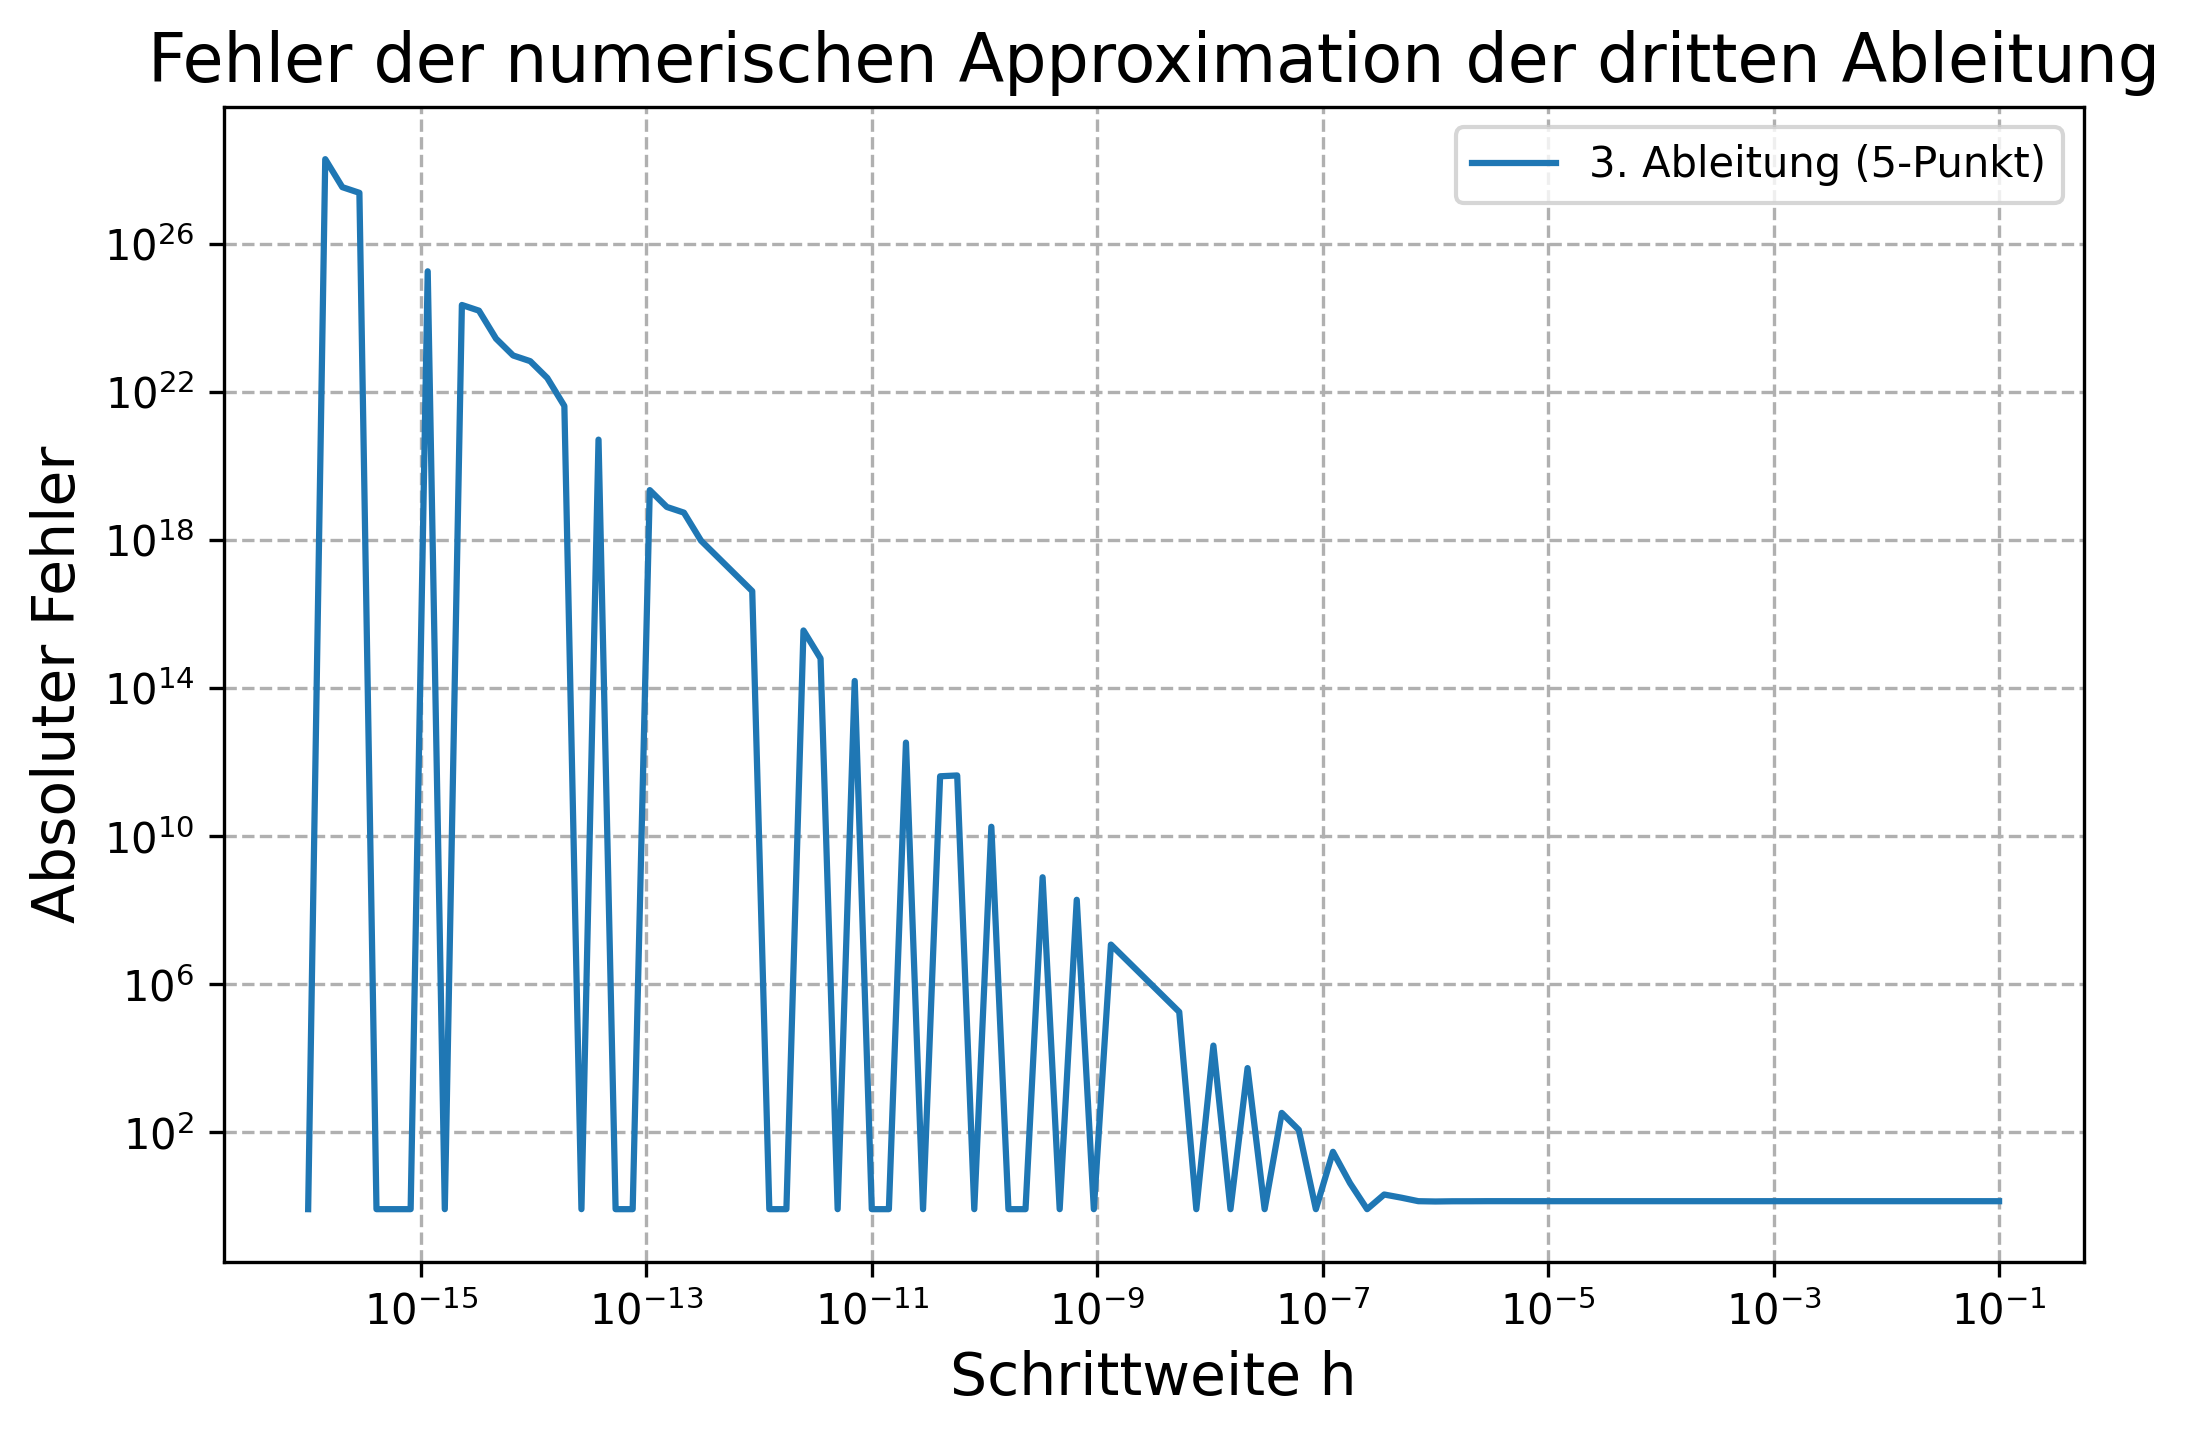
\includegraphics[width=0.8\textwidth]{papers/step/img/dritte_ableitung_vergleich.png}
	\caption{Absoluter Fehler der numerischen Approximation der dritten Ableitung von $\sin(x)$ in Abhängigkeit von der Schrittweite $h$.}
	\label{fig:dritte_ableitung_vergleich}
\end{figure}
Selbst für kleine Schrittweiten wird der Fehler der numerischen Approximation sehr gross, was die Grenzen klassischer Finite-Differenzen-Methoden aufzeigt.
Es existieren jedoch moderne Verfahren, die gezielt darauf abzielen, diese Fehlerquellen zu minimieren oder vollständig zu umgehen. 
Sie ermöglichen es, Ableitungen sehr präzise zu berechnen, selbst wenn die Schrittweiten klein gewählt werden müssen oder sehr hohe Genauigkeit gefordert ist. 
Besonders bei höheren Ableitungen, wie der dritten oder vierten Ableitung, sind diese Ansätze essentiell, da klassische Differenzenmethoden hier numerisch instabil werden.
Im folgenden Abschnitt werden zwei solcher Ansätze vorgestellt, die jeweils den Diskretisierungs- bzw. den Rundungsfehler adressieren und somit die Limitationen klassischer Differenzenmethoden überwinden.

%Die bisher diskutierten Fehlerquellen – Diskretisierungsfehler durch den Abbruch der Taylor-Reihe und Rundungsfehler aufgrund der endlichen Gleitkommaarithmetik – limitieren die Genauigkeit klassischer Differenzenquotienten. 
%In der Praxis existieren jedoch moderne Verfahren, die gezielt darauf abzielen, diese Fehlerquellen zu minimieren oder vollständig zu umgehen. 
%Sie ermöglichen es, Ableitungen sehr präzise zu berechnen, selbst wenn die Schrittweiten klein gewählt werden müssen oder sehr hohe Genauigkeit gefordert ist. 
%Im folgenden Abschnitt werden zwei solcher Ansätze vorgestellt, die jeweils den Diskretisierungs- bzw. den Rundungsfehler adressieren und somit die Limitationen klassischer Differenzenmethoden überwinden.
















%
%Die klassische Methode zur numerischen Berechnung von Ableitungen ist die \textbf{Finite-Differenzen-Methode}. Dabei approximiert man die Ableitung einer Funktion $f(x)$ durch kleine Änderungen in $x$:
%
%\[
%f'(x) \approx \frac{f(x+h) - f(x)}{h}
%\]
%
%\textbf{Probleme:} 
%\begin{itemize}
%	\item Fehler durch Rundung und Subtraktion (Cancellation Error) bei sehr kleinen $h$
%	\item Trade-off zwischen Schrittweite $h$ und Genauigkeit
%\end{itemize}
%
%\begin{verbatim}
%	import numpy as np
%	
%	def f(x):
%	return np.sin(x)
%	
%	x0 = 1.0
%	h = 1e-5
%	
%	finite_diff = (f(x0 + h) - f(x0)) / h
%	print("Finite Difference Approx:", finite_diff)
%	print("Analytical Derivative:", np.cos(x0))
%\end{verbatim}
%
%\section{Complex Step Derivative}
%
%Die \textbf{Complex-Step-Methode} nutzt die analytische Fortsetzung von $f$ ins Komplexe:
%
%\[
%f'(x) \approx \frac{\operatorname{Im}[f(x + i h)]}{h}
%\]
%
%\textbf{Vorteile:}
%\begin{itemize}
%	\item Sehr hohe Genauigkeit
%	\item Schrittweite $h$ kann extrem klein gewählt werden
%\end{itemize}
%
%\begin{verbatim}
%	def complex_step_derivative(f, x, h=1e-20):
%	return np.imag(f(x + 1j*h)) / h
%\end{verbatim}
%
%\section{Automatic Differentiation (AD)}
%
%Automatic Differentiation berechnet Ableitungen exakt, indem die Kettenregel systematisch auf alle Rechenoperationen angewendet wird.  
%Es gibt zwei Modi:
%\begin{itemize}
%	\item \textbf{Forward Mode}: effizient bei wenigen Eingaben und vielen Ausgaben
%	\item \textbf{Reverse Mode}: effizient bei vielen Eingaben und wenigen Ausgaben (typisch für ML)
%\end{itemize}
%
%\begin{verbatim}
%	import jax.numpy as jnp
%	from jax import grad
%	
%	def f_jax(x):
%	return jnp.sin(x) * jnp.exp(x)
%	
%	x0_jax = 1.0
%	df_dx = grad(f_jax)(x0_jax)
%	print("Automatic Differentiation (JAX) Derivative:", df_dx)
%\end{verbatim}
%
%\section{Anwendungsbeispiel: Gradientbasiertes Lernen}
%
%\begin{verbatim}
%	from jax import grad
%	import jax.numpy as jnp
%	
%	def loss(w):
%	return (w**2 - 4*w + 4)
%	
%	w = 0.0
%	learning_rate = 0.1
%	
%	for i in range(10):
%	g = grad(loss)(w)
%	w -= learning_rate * g
%	print(f"Step {i}: w = {w}, loss = {loss(w)}")
%\end{verbatim}
%
%\section{Ausblick: Höhere Ableitungen}
%
%AD kann auch für höhere Ableitungen verwendet werden (z. B. Hessian-Matrizen):
%
%\begin{verbatim}
%	from jax import jacfwd, jacrev
%	import jax.numpy as jnp
%	
%	def f_hessian(x):
%	return x[0]**2 + x[0]*x[1] + x[1]**2
%	
%	x_vec = jnp.array([1.0, 2.0])
%	hessian = jacfwd(jacrev(f_hessian))(x_vec)
%	print("Hessian Matrix:\n", hessian)
%\end{verbatim}
%
%\section{Zusammenfassung}
%
%\begin{tabular}{l|l|l}
%	Methode & Vorteil & Nachteil \\
%	\hline
%	Finite Differences & Einfach, universell & Subtraktionsfehler, Schrittweitenproblem \\
%	Complex Step & Sehr genau, einfach zu implementieren & Funktion muss komplexwertig sein \\
%	Automatic Differentiation & Exakte Ableitung, skalierbar & Framework nötig, Overhead bei sehr komplexen Funktionen \\
%\end{tabular}